\section{Hardwarearkitektur}
I den følgende sektion om hardwarearkitektur beskrives opbygningen af systemet ved brug af sysML. Hardwarearkitekturen indholder diagrammerne BDD og IBD samt en kort forklaring af disse. For ydeligere information om interaktionen i systemet henvises til dokumentet arkitektur og design for flere detaljer. Dette dokument indeholder bloktabel og signaltabel, der fortæller om alle blokke, porte og signaler, der ses i diagrammerne. Yderligere information omkring valg af elementer i systemet findes i dokumentet analyse, som findes i bilaget.

\subsection{BDD}
Et BDD viser opbygningen af et system med brug af blokke. Nedenstående diagram på figur \vref{fig:BDD} viser opbygningen af vores blodtrykssytem, der består af en række forskellige elementer. 

\begin{figure}[h!]
	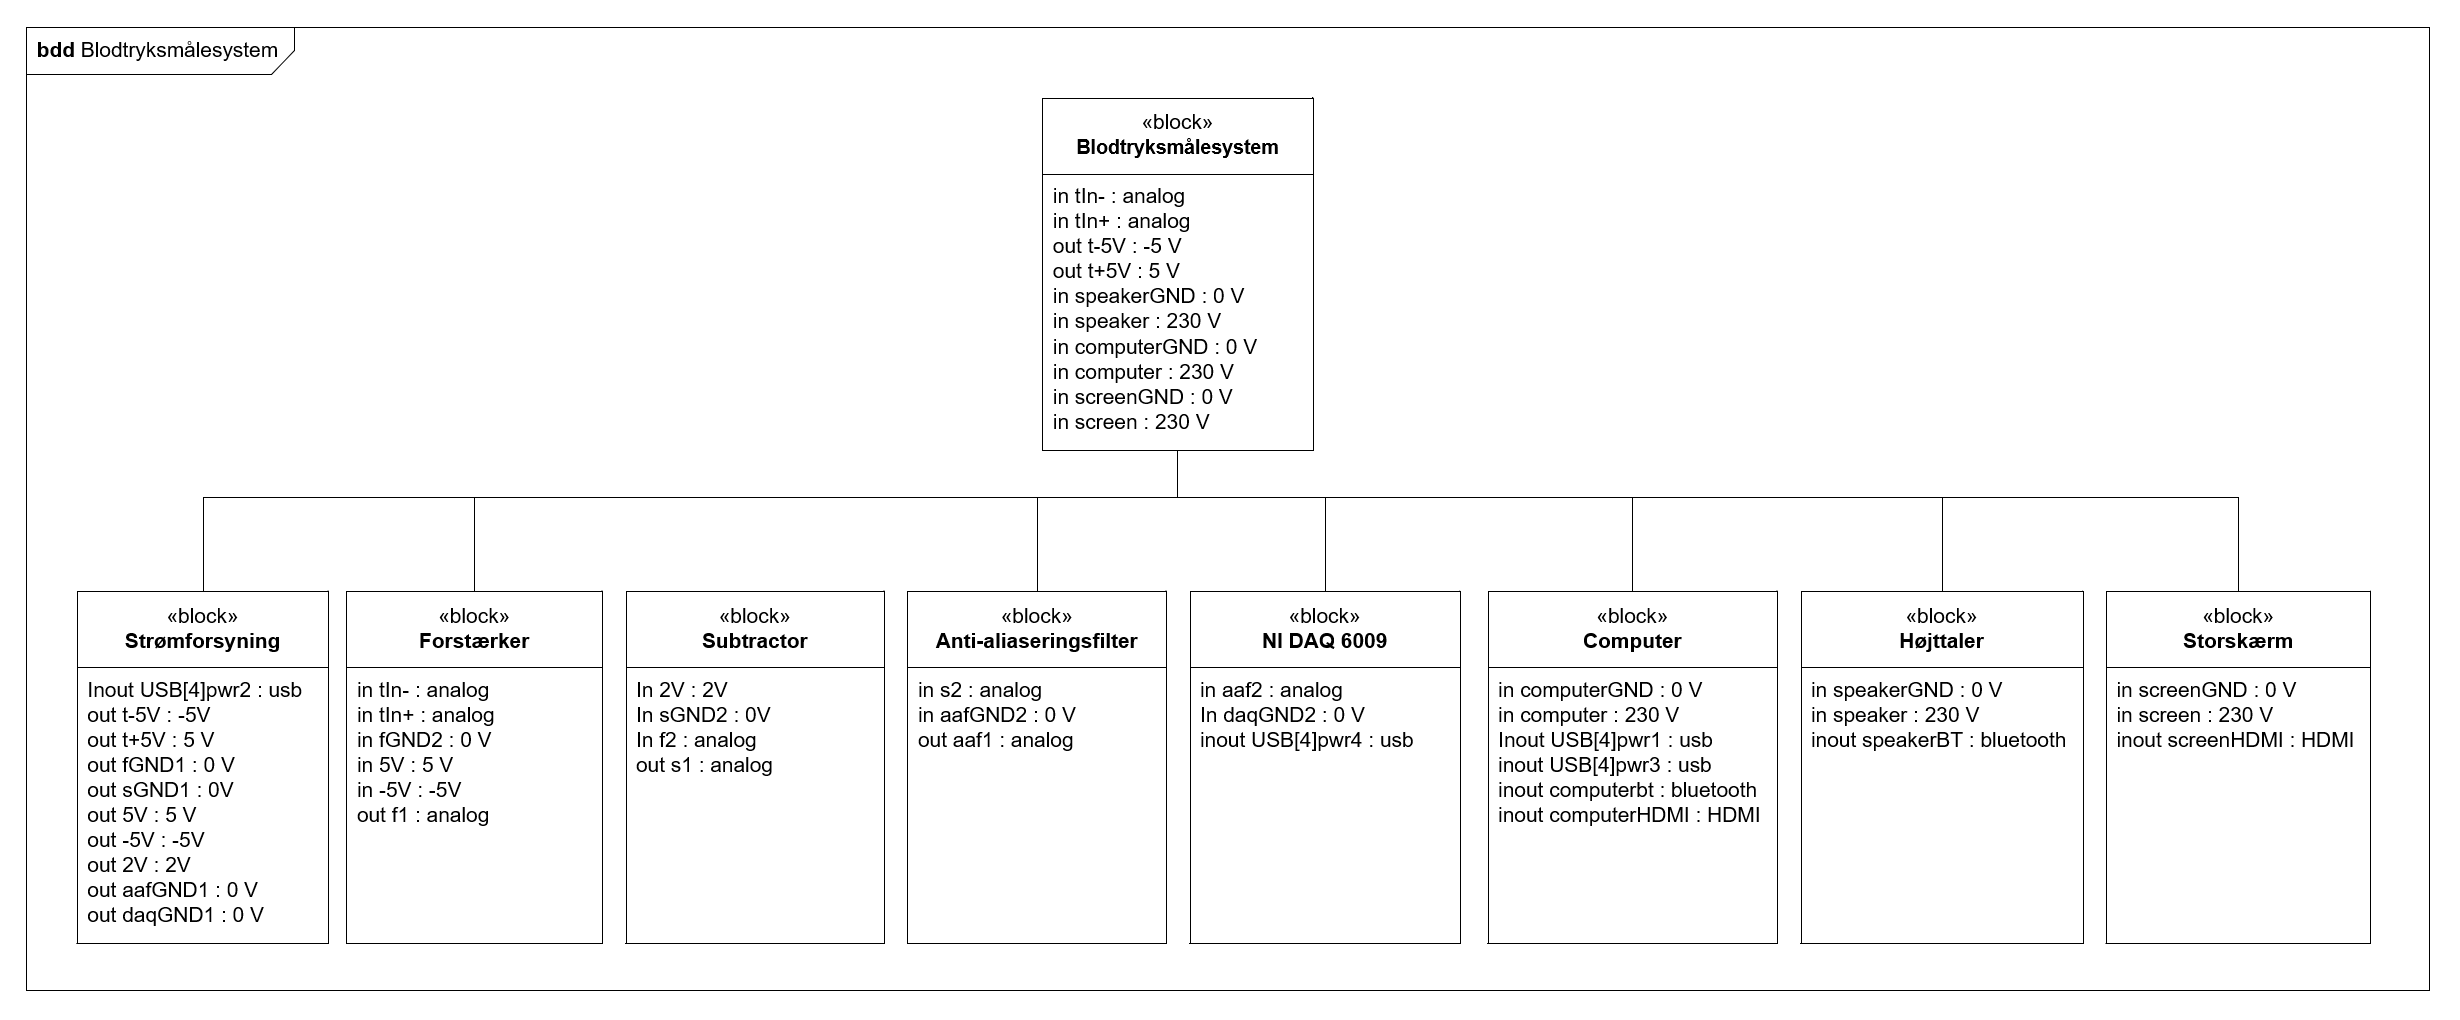
\includegraphics
	[width=1\linewidth]{Arkitektur_og_design/Hardwarearkitektur/BDD_faerdig}
	\caption{BDD Blodtrykmålesystem}
	\label{fig:BDD}
\end{figure}

På BDD'et ses de forskellige elementer, der er er en del af blodtrykmålesystemet. Den øverste blok $"$Blodtryksmålesystem$"$ viser systemets interaktioner med udefrakommende objekter. I denne blok findes tilslutningen til tryktransduceren, som ikke er en del af selve systemet. I blokken findes også tilslutningen af strøm til henholdsvis computer, højtaler og storskærm. 

På diagrammet ses også otte blokke, der repræsenterer de forskellige dele af systemet. Systemet består altså af en strømforsyning, en forstærker, en subtractor, et filter, en AD-Converter, en computer, en højtaler og en storskærm. Strømforsyningen giver strøm til tryktransducer, forstærker og subtractor og udgøres af Analog Discovery. Forstærker, subtractor og filter er designet til systemet i forbindelse med projektet. Mere info om disse elementer i afsnit .... om design af hardware.

\clearpage

\subsection{IBD}
Et IBD viser en mere detaljeret opbygning af et system fordi alle forbindelser mellem blokkene, der findes i BDD'et er tegnet. På nedenstående figur \vref{fig:IBD} ses derved opbygningen af blodtryksmålesystemet inklusiv alle forbindelser mellem blokkene.

\begin{figure}[h!]
	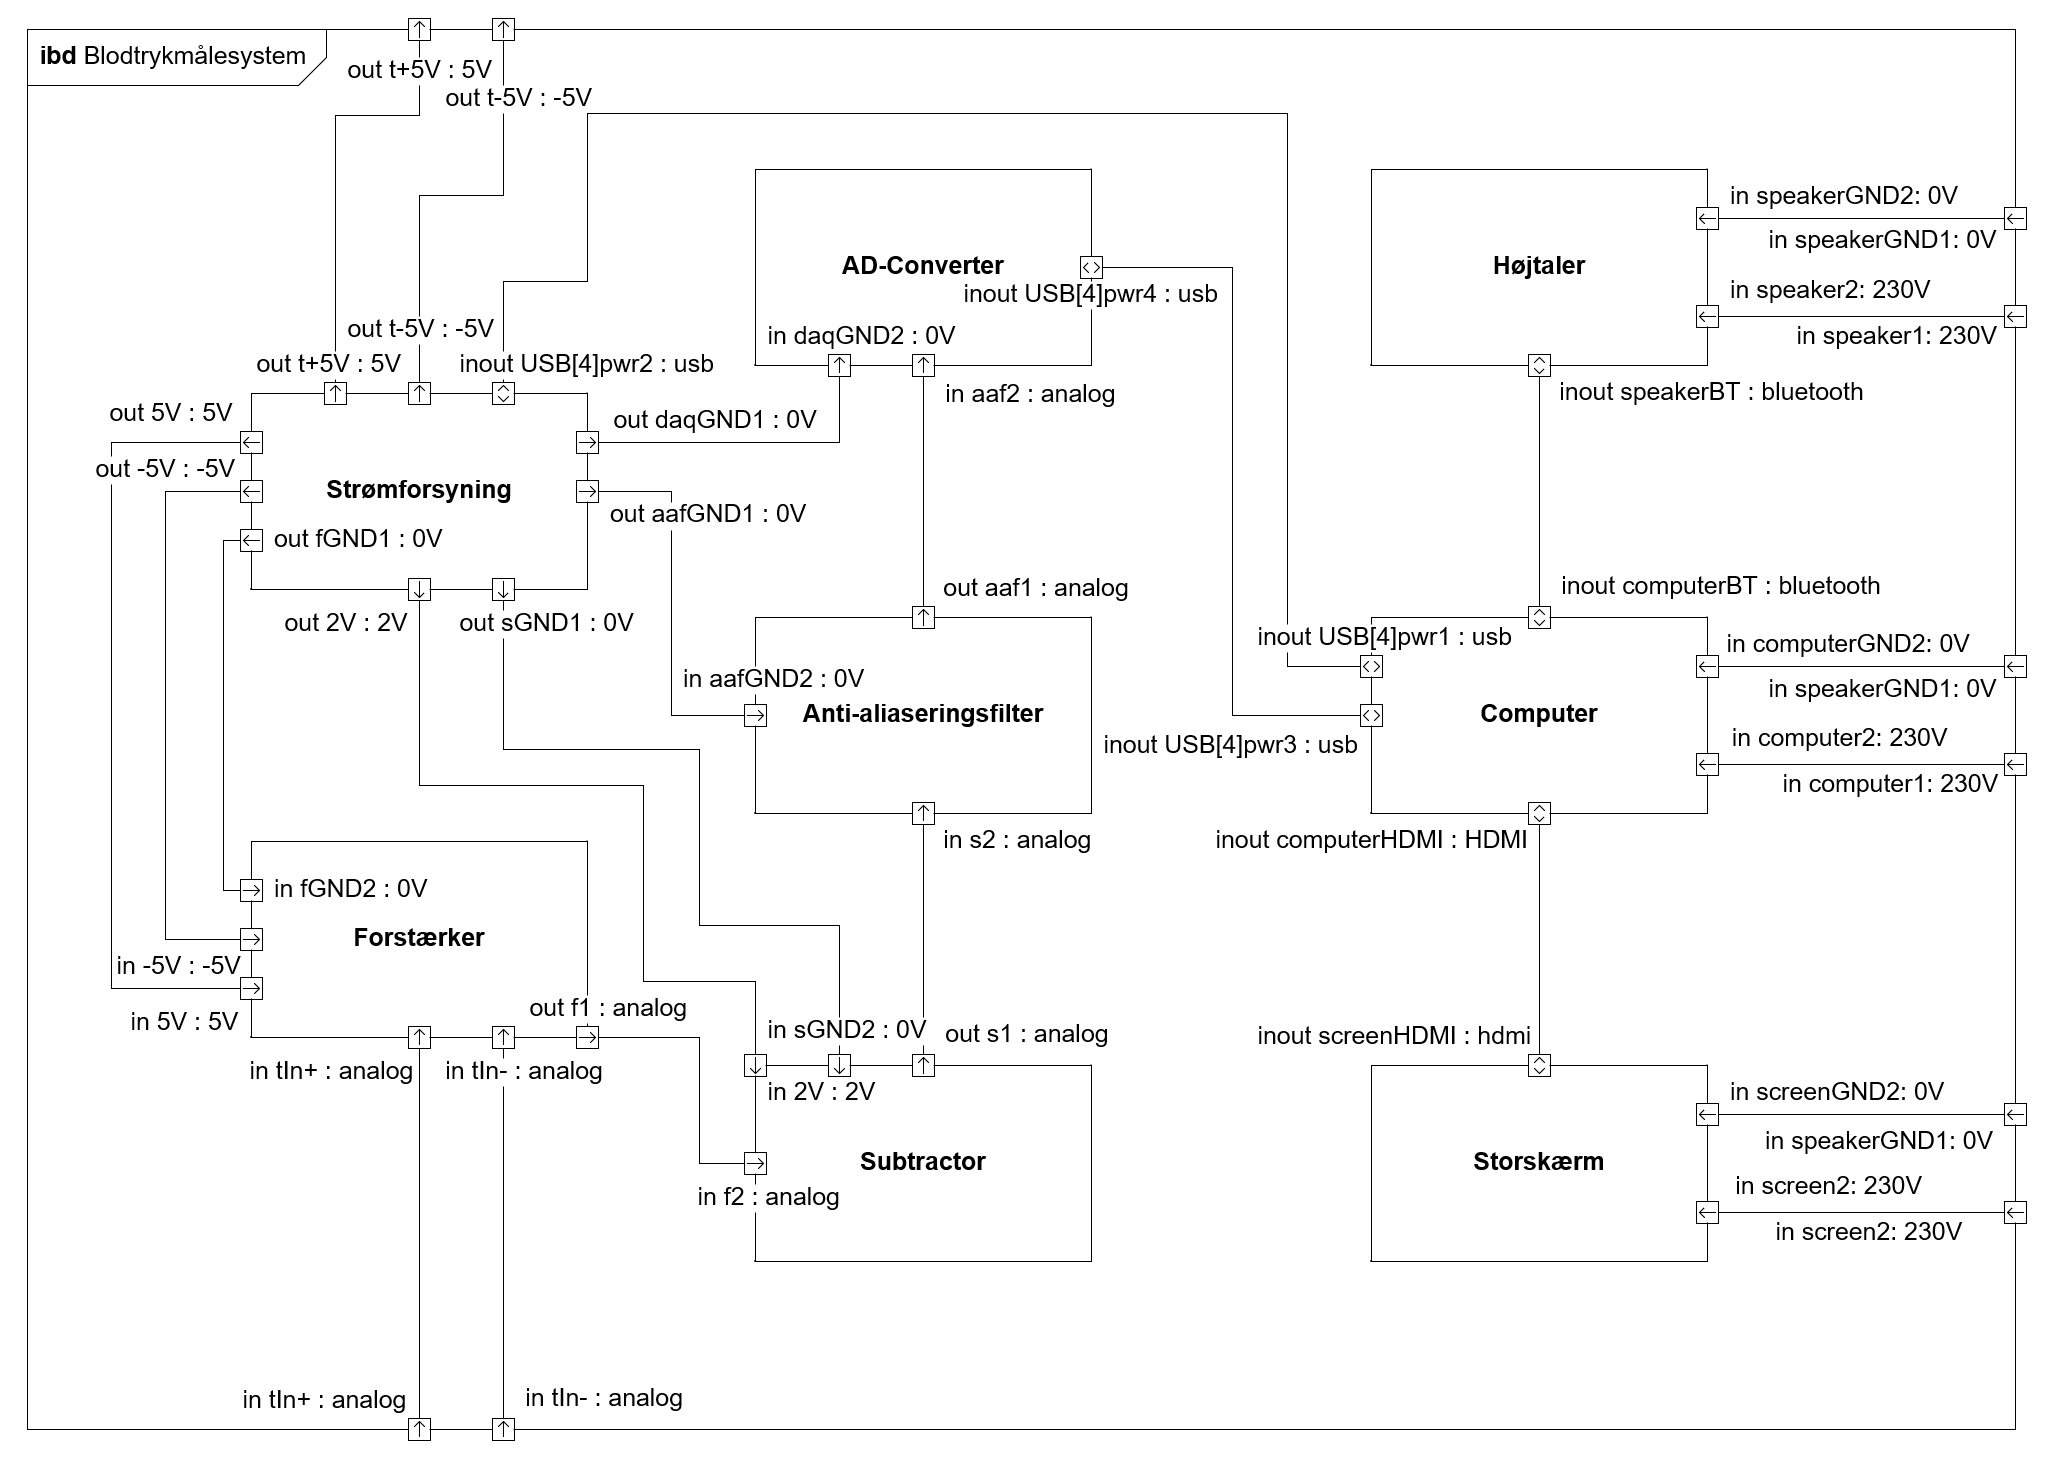
\includegraphics
	[width=1\linewidth]{Arkitektur_og_design/Hardwarearkitektur/IBD_faerdig}
	\caption{IBD Blodtrykmålesystem}
	\label{fig:IBD}
\end{figure} 

Den yderste ramme omkring diagrammet illustrerer den øverste blok $"$Blodtryksmålesystem$"$ på figur \vref{fig:BDD}. Her ses det tydeligt hvordan nogle af blokkene interagerer med objekter uden for selve systemet fordi forbindelserne er tegnet ud til rammen. Hver port har et unikt portnavn. IBD'et er med til at forbinde portnavnene fra BDD'et sammen, så overblikket over systemet som en helhed giver mening. 

\clearpage